\section{Using Algebraic Geometry to Assist in Abstraction refinement}
\subsection{Previous work}
Traditional methods to analyze sequential circuits require state variable encoding
as well as a complete/exact state enumeration with the initial state and transition function.
With the size of modern sequential circuits increasing, it is infeasible to apply conventional methods
any longer. Abstraction is a technique to minimize the state space representation by combining states with certain 
similarities. Sometimes it can effectively lower the number of states that require analysis by orders of magnitude,
without affecting the properties we need to verify.

At first, abstraction was done manually by designers. In 2000, E. Clarke \cite{clarke2000counterexample}
proposed an automated abstraction: first,
initial abstraction is set up by dividing variables to different clusters based on transition conditions;
then, an ordinary model checking is applied on this abstraction. If a counterexample is detected, 
it is further checked to be concrete or not. For a false abstract state or a spurious path 
, the initial abstraction is refined by further splitting the false abstract state. 
A heuristic algorithm keeps refining the abstraction until a real counterexample is found or the 
property is verified. This technique is based on binary decision diagrams (BDDs), which implies a
potential risk of memory explosion; meanwhile it still requires an initial abstraction to start with.

In 2004 L. Zhang and M. Hsiao \cite{zhang2005design} proposed another abstraction method based on CNF-SAT.
This paper uses simplest latch abstraction -- by removing "irrelevant" latches from the analysis. 
The key idea is to pick those ``irrelevant" latches (variables in $k$-bounded model checking, $k$-BMC) 
according to SAT/UNSAT analysis from the $k$-BMC. It improves the $k$-BMC procedure\cite{biere1999symbolic}: 
linear temporal logic (LTL) properties to check for can be translated to a (big) CNF formula and fed to a SAT solver. 
If SAT, a concrete counterexample is found. 
If UNSAT, the original method increases the bound $k$. In Zhang's paper, the clauses for UNSAT 
(UNSAT cores\footnote{UNSAT core is a subset of the original CNF clauses which are also unsatisfiable.})
are checked for variables that do not appear.
Thus an abstracted model is obtained and checked with the original property. If the abstracted model checking fails, 
then bound $k$ is increased. This method still has disadvantages: it is counterexample-independent,
which means it cannot utilize information from invariants.

In 2005, H. Jain et al.\cite{HimanshuDAC2005} improved the abstraction refinement technique of \cite{clarke2000counterexample},
where they use CNF-SAT to perform the refinement instead of using BDDs. The new approach is applied to verify RTL Verilog
and was known to be successful.

Abstraction usually means over-approximation, i.e. properties that are true on the abstracted machine
are also valid for the original states. Craig's interpolation is a sort of abstraction which may be either
over-approximation or under-approximation. In 2003, K. McMillan used Craig's interpolation to improve 
$k$-BMC \cite{mcmillan2003interpolation}. Initially a $k$-length path to failure state $F$ is picked and transformed to 
a CNF formula, then split at first transition into a prefix and a suffix. An interpolation $P$ is computed
between the prefix and suffix. $P$ over-approximates 1-step reachable states, and under-approximates states 
that cannot reach $F$ in $k$ steps. If no counterexample is exposed, the path is split again at the second
transition; in this way a precise abstraction can be found for all reachable states.

$k$-BMC with interpolation is a purely incremental model checking approach, and the interpolation procedure relies
on UNSAT core analysis. To overcome these weaknesses, a hybrid model checker named as IC3 is developed 
\cite{bradley2011sat} \cite{bradley2011incremental}. IC3 works incrementally to find out inductive subclauses
of negations of reached states, meanwhile it is monolithic when computing over-approximations to sets of reachable
states within $1,2,\dots,k$ steps. It is proved to be more efficient than interpolation based model checking
although using similar mechanisms.

\subsection{Exploiting UNSAT cores for abstraction refinement}
By exploring previous work, we learn that most state-of-art abstraction refinement techniques require 
information mining from UNSAT proofs of intermediate abstractions. 
Here we use an abstraction refinement algorithm from \cite{zhang2005design} to explain that how an UNSAT proof is
utilized in such techniques.

\begin{algorithm}[hbt]
\SetAlgoNoLine
	\KwIn{$M$ is the original machine, $p$ is the property to check, $k$ is the number of steps in $k$-BMC}
  $k = $ InitValue\;
  \eIf{$k$-BMC$(M,p,k)$ is \textbf{SAT}}
  {
	\Return{``Found error trace"}
  }
  {
	Extract UNSAT proof $\mathcal P$ of $k$-BMC\;
	$M' = $ \textit{ABSTRACT}$(M,\mathcal P)$\;
  }
  \eIf{MODEL-CHECK$(M',p)$ returns \textbf{PASS}}
  {
	\Return{``Passing property"}
  }
  {
	Increase bound $k$\;
	goto Line 2\;
  }
\caption {Abstraction refinement using $k$-BMC}\label{alg:absrefine}
\end{algorithm}
\begin{figure}[hbt]
\centering{
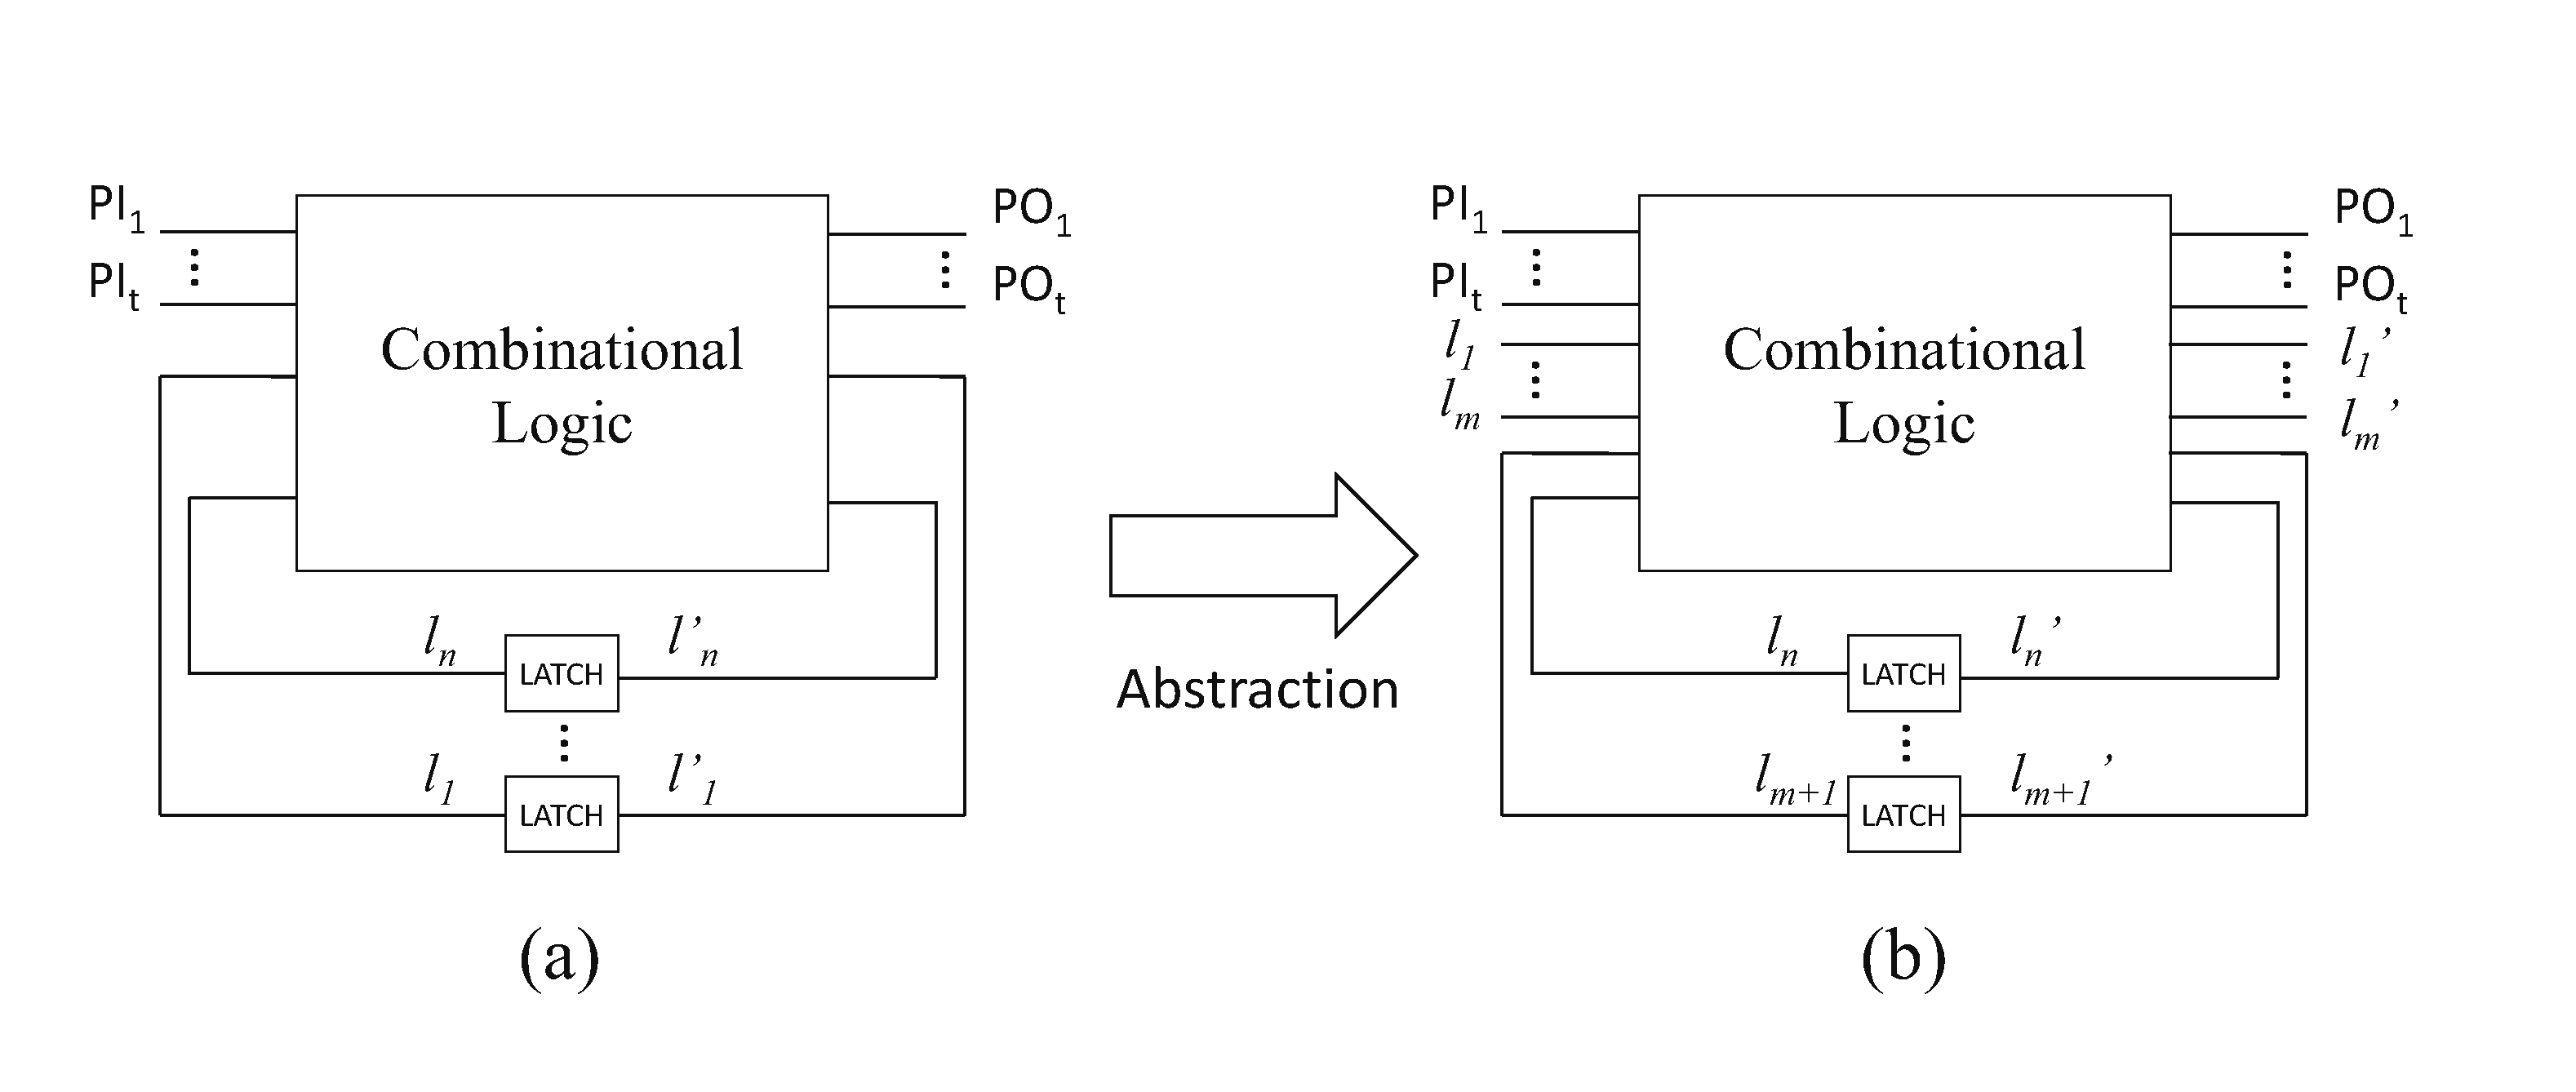
\includegraphics[width=5.5in]{./refine.eps}
\caption{Abstraction by reducing latches}
\label{fig:refine}}
\end{figure}
Assume that we are given a sequential circuit with $n$ latches as shown in Fig.\ref{fig:refine}(a). 
This circuit can be modeled as a Mealy machine $M$ and the states $s$ can be explicitly encoded by bit-level latch variables 
$l_1,\dots,l_n$. Algorithm \ref{alg:absrefine} describes an approach to check if machine $M$ violates property $p$.
This algorithm relies on $k$-BMC technique, which works on the basis of CNF-SAT solving.
The $k$-BMC represents the initial states $I$, the transition relation $T$ and property $p$ as CNF formulas.

The first ``if-else" branch in Algorithm \ref{alg:absrefine} can be
explained as: we check if the conjunction of formulas 
$$I(s_0)\land \bigwedge_{i=0}^{k-1}T(s_i,s_{i+1}) \land \neg p$$
is $SAT$ or not, where $s_i$ denotes the set of reached states in $i$-th time-frame. If the result is
$SAT$, then a counterexample is found that violates property $p$. If the result is $UNSAT$, we cannot
assert that $p$ is satisfied for the original machine $M$ because we only unrolled $M$ for a given specific number of time-frames
without any fixpoint detected.
In this algorithm, we analyze the UNSAT core composed by a set of clauses whose conjunction is $UNSAT$.
If there are some latch variables not included in this UNSAT core (denoted by $L_{abs}$), then we can assert that the evaluations of 
these variables will not affect the unsatisfiability of original formula. Therefore, we can ignore them in the abstracted model.
In practice, we turn these latches into primary inputs/outputs as shown in Fig.\ref{fig:refine}(b) ($L_{abs} = \{l_1,\dots,l_m\}$).


The second ``if-else" branch means: if we do an ordinary model checking on the abstracted machine $M'$ and find no
error trace, we can assert that property $p$ also holds on the original machine $M$. The reason of this assertion is that
the abstracted states represented using abstracted latches cover the original states, which means $M'$ is an over-approximation
of $M$, such that $(M'\implies p) \implies (M\implies p)$. If we find a violation on abstracted machine, then this
abstracted model is not a suitable model to check $p$, so we have to increase the bound $k$ to find a finer abstraction.

It is clear that UNSAT cores play an important role in abstraction refinement approaches. In \cite{zhang2005design}
the UNSAT core is extracted using a conventional CNF-SAT solver, which will encounter the ``bit-blasting" problem
when the size of datapath (number of latches in Fig.\ref{fig:refine}) is very large. \textbf{Here we propose a totally new 
method based on Gr\"obner basis computation to extract UNSAT cores, and we believe it may become an efficient 
method according to the following observation based on our experience:}

% {\it Gr\"obner basis is more suitable for UNSAT problems because of following theorem:}
{\it While computing GB over finite fields is exponential in the number of variables, GB  computation 
is observed to be more efficient for UNSAT problems.} 
The reason is discussed as follows:
\begin{Theorem}
{\bf Weak Nullstellensatz:} Given ideal $J\subset \mathbb F[x_1,\dots,x_n]$, its variety over algebraic closure
of field $\mathbb F$ is empty if and only if its reduced Gr\"obner basis contains only one generator ``1".
$${\bf V}_{\overline{\mathbb F}}(J) = \emptyset \Longleftrightarrow reducedGB(J) = \{1\}$$
\end{Theorem}
It is well known that using Buchberger's algorithm and its variations to compute a GB has a very high
time complexity and is usually not practicable. One reason is that the size of GB may explode even if the term
ordering is carefully chosen. However if the reduced GB is 1, which means every term in the original polynomials
will be canceled, the degree of remainders when computing GB with Buchberger's algorithm will be limited. 
Thus the number of polynomials in non-reduced GB is much smaller than usual.
Instead of applying polynomial calculus to SAT solving, it may be more efficient to try it for UNSAT
problems.

\subsection{A demonstration of our conjecture}
One  important research topic about UNSAT problems is to identify UNSAT cores efficiently.
An UNSAT core in a CNF formula denotes a subset of clauses which is still unsatisfiable. Here
we re-define this concept in algebraic geometry:
\begin{Definition}
Assume a set of polynomials $F$ and its subset $F_s\subset F$. If ${\bf V}(\langle F\rangle) = {\bf V}
(\langle F_s\rangle) = \emptyset$, we call $F_s$ an {\bf UNSAT core} of $F$. Additionally, if
$F_s$ contains no other UNSAT core, we call it a {\bf minimal} UNSAT core.
\end{Definition}

We  conjecture that based on observation of Buchberger's algorithm's execution, an UNSAT core can be identified.
\begin{Conjecture}
Buchberger's algorithm picks pairs of polynomials from a given set, computes their S-poly, then reduces this S-poly
with the given set of polynomials. If the remainder is non-zero,
it is added to the set of polynomials.
By tracking S-poly computations and multivariate divisions that lead to remainder 
1, we can obtain an UNSAT core. Moreover, we can identify a minimal UNSAT core with one-time
 execution of Buchberger's algorithm.
\end{Conjecture}
\begin{Example}
A SAT problem is described with 8 CNF clauses:

\begin{minipage}[h]{0.3\textwidth}
\begin{align*}
&c_1: \bar{a}\lor\bar{b}\\
&c_2: a\lor\bar{b}\\
&c_3: \bar{a}\lor b\\
&c_4: a\lor b
\end{align*}
\end{minipage}
\begin{minipage}[h]{0.7\textwidth}
\begin{align*}
&c_5: x\lor y\\
&c_6: y\lor z\\
&c_7: b\lor \neg y\\
&c_8: a\lor x\lor \neg z
\end{align*}
\end{minipage}

% \begin{align*}
% &\bar{a}\lor\bar{b}\\
% &a\lor\bar{b}\\
% &\bar{a}\lor b\\
% &a\lor b\\
% &x\lor y\\
% &y\lor z\\
% &b\lor \neg y\\
% &a\lor x\lor \neg z
% \end{align*}
Using Boolean to polynomial mappings given in Table \ref{tab:booltof4}, we can transform them to a set of
polynomials $F$ over ring $\mathbb F_2[a,b,x,y,z]$:

\begin{minipage}[h]{0.4\textwidth}
\begin{align*}
&f_1:ab\\
&f_2:ab+a\\
&f_3:ab+b\\
&f_4:ab+a+b+1
\end{align*}
\end{minipage}
\begin{minipage}[h]{0.6\textwidth}
\begin{align*}
&f_5:xy+y+x+1\\
&f_6:yz+y+z+1\\
&f_7:by+y\\
&f_8:axz+az+xz+z
\end{align*}
\end{minipage}
% \begin{align*}
% &f_1:ab\\
% &f_2:ab+a\\
% &f_3:ab+b\\
% &f_4:ab+a+b+1\\
% &f_5:xy+y+x+1\\
% &f_6:yz+y+z+1\\
% &f_7:by+y\\
% &f_8:axz+az+xz+z
% \end{align*}
We compute its GB using Buchberger's algorithm with lexicographic term ordering $a>b>x>y>z$.
Since this problem is UNSAT, we will stop when ``1" is added to GB.
\begin{enumerate}
\item First we compute $Spoly(f_1,f_2)\xrightarrow{F}_{+} r_1$, remainder $r_1$ equals to $a$;
\item Update $F=F\cup r_1$;
\item Next we compute $Spoly(f_1,f_3)\xrightarrow{F}_{+} r_2$, remainder $r_2$ equals to $b$;
\item Update $F=F\cup r_2$;
\item We can use a directed acyclic graph (DAG) to represent the process to get $r_1,r_2$, as Fig.\ref{fig:UNSAT}(a) shows;
\item Then we compute $Spoly(f_1,f_4) = s_3= a+b+1$, obviously $a+b+1$ can be reduced (multivariate divided) by
$r_1$ , the intermediate remainder $r_3 = b+1$. It can be immediately divided by $r_2$, and the remainder is ``1", we
terminate the Buchberger's algorithm;
\item We draw a DAG depicting the process through which we obtain remainder ``1" as shown in Fig.\ref{fig:UNSAT}(b). 
From leaf ``1" we backtrace the graph to roots $f_1,f_2,f_3,f_4$. They constitute an UNSAT core for this problem
as these polynomials are the ``causes" of unsatisfiability of original set of clauses.
\end{enumerate}
\end{Example}
\begin{figure}[hbt]
\centering{
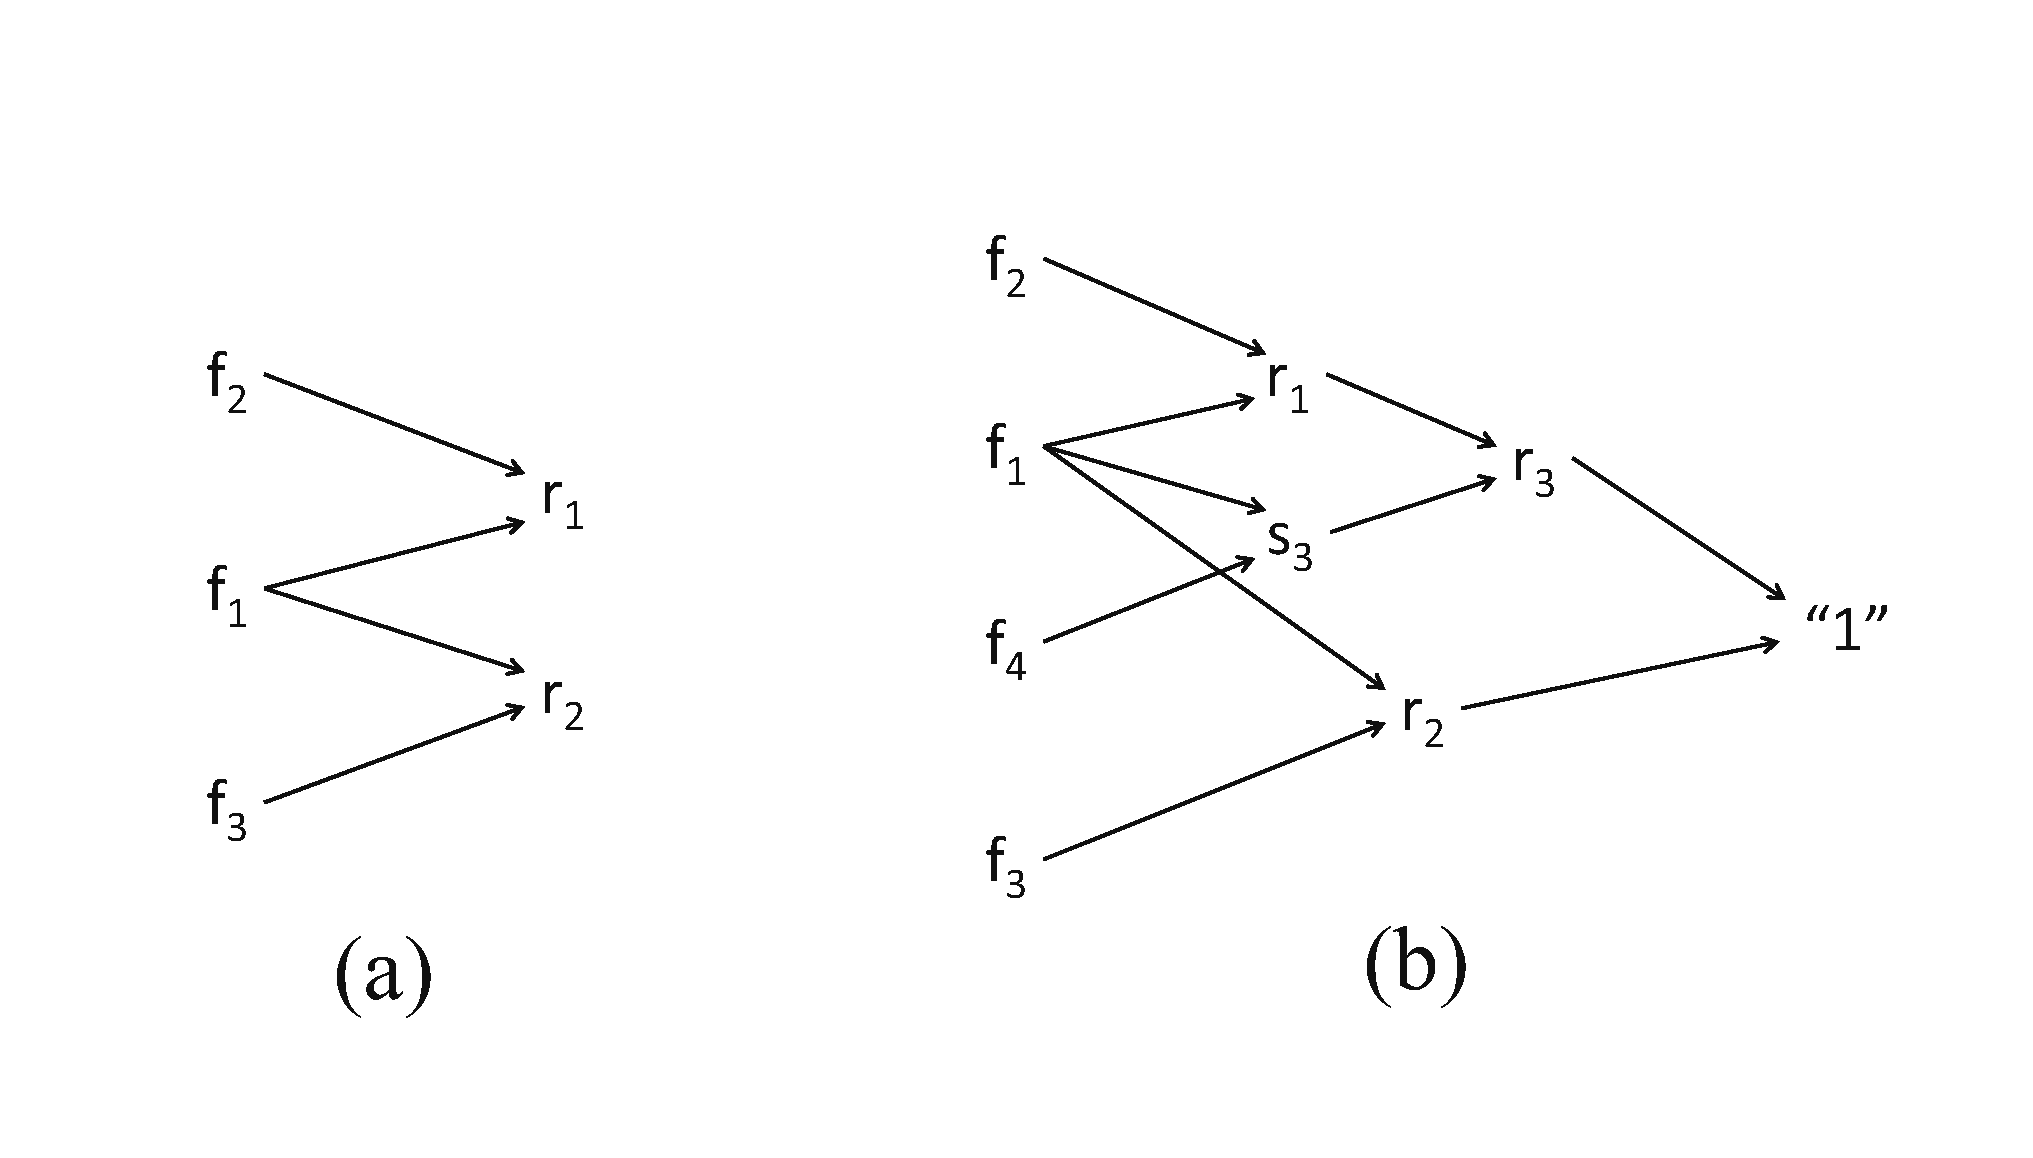
\includegraphics[width=4.5in]{./UNSAT.eps}
\caption{DAG representing Spoly computations and multivariate divisions}
\label{fig:UNSAT}}
\end{figure}
% We conclude our approach as follows: i) Keep track of all $Spoly(f_i,
% f_j)\xrightarrow{f_1, \dots, f_s}_+ r$; ii) mark $f_i, f_j$ if $r\neq
% 0$; iii) Mark those $f_l$'s that have leading terms that cancel
% monomial terms in $Spoly(f_i, f_j)$; iv) Build a DAG recording all reductions including Spoly computations
% and multivariate divisions; v) Once $1\in J$ is
% detected, traverse the graph to identify all the marked polynomials that were
% used in obtaining this unit element. These polynomials constitute the
% core.

We conclude our approach as a conjecture algorithm (Algorithm \ref{alg:UNSAT}). 

\begin{algorithm}[hbt]
\SetAlgoNoLine
	\KwIn{A set of polynomials $F = \{f_1,f_2,\dots,f_s\}$}
	\KwOut{An UNSAT core $\{f_{m_1},f_{m_2},\dots,f_{m_t}\}$}
\Repeat{$r_l == 1$}
{
	Pick a pair $f_i,f_j\in F$ that has never been computed S-poly\;
	\If{$Spoly(f_i,f_j)\xrightarrow{F}_+ r_l \neq 0$}
	{
		$F = F\cup r_l$\;
		Create a DAG $G_l$ with $f_i,f_j$ as roots, $r_l$ as leaf, recording the S-poly, all intermediate remainders and $f_k\in F$ that cancel monomial terms in the S-poly\;
	}
}
Backward traverse the DAG for remainder ``1", replace $r_l$ with corresponding DAG $G_l$\;
\Return{All roots}
\caption {Extract UNSAT core using a variation of Buchberger's algorithm}\label{alg:UNSAT}
\end{algorithm}

\subsection{Research objective}
i) To prove that the algorithm is concrete and complete: it can always abstract an UNSAT core;

ii) To design an algorithm to find a minimal UNSAT core;

iii) Run the algorithm at word level, to find UNSAT proofs for word-level variables in $\Fkk$, which 
can help word-level abstraction refinement procedure.

% If we start with other term orderings, we may get a larger UNSAT core. By dynamically adjusting
% term ordering and re-calculate GB, we can get new UNSAT core with smaller size, until
% we find minimal UNSAT core or expire runtime limit.